
\section{Ejercicio 6}

\subsection{Introducción}

En este ejercicio se realizará el diseño de un circuito que adapta una señal de tensión proveniente de un sensor de temperatura LM324. 
Luego, se implementará el mismo en un PCB y se analizarán los resultados obtenidos.

\subsection{Diseño del circuito}

Como primer paso se deben definir las entradas y salidas del sistema para poder comenzar con su diseño. Respecto a la entrada, la fuente de la misma es el sensor de temperatura LM324.
 Según se pudo consultar en su datasheet, la ganancia del mismo es de $100 \frac{mV}{°C}$.Por otro lado, el rango de temperaturas especificado de funcionamiento del circuito va desde $35°C$ hasta $45°C$.
 Luego, el rango de tensiones de entrada es de $350mV$ a $450mV$, lineal respecto de la temperatura. El rango de salida del circuito está comprendido entre $0V$ y $5V$, a  $35°C$ y $45°C$ respectivamente. 

 
 Como se puede observar, tanto la entrada como la salida del circuito son rangos lineales, por lo que la adaptación implica solamemte un escalamiento y un corrimiento aplicados sobre la señal de entrada.
  Teniendo en cuenta los circuitos típicos observados en clase se decidió emplear un sumador inversor conectado en cascada a un amplificador inversor, como se puede observar en la figura~\ref{fig:EJ6_circuito}.  
  
\begin{figure}[H]
    \centering
    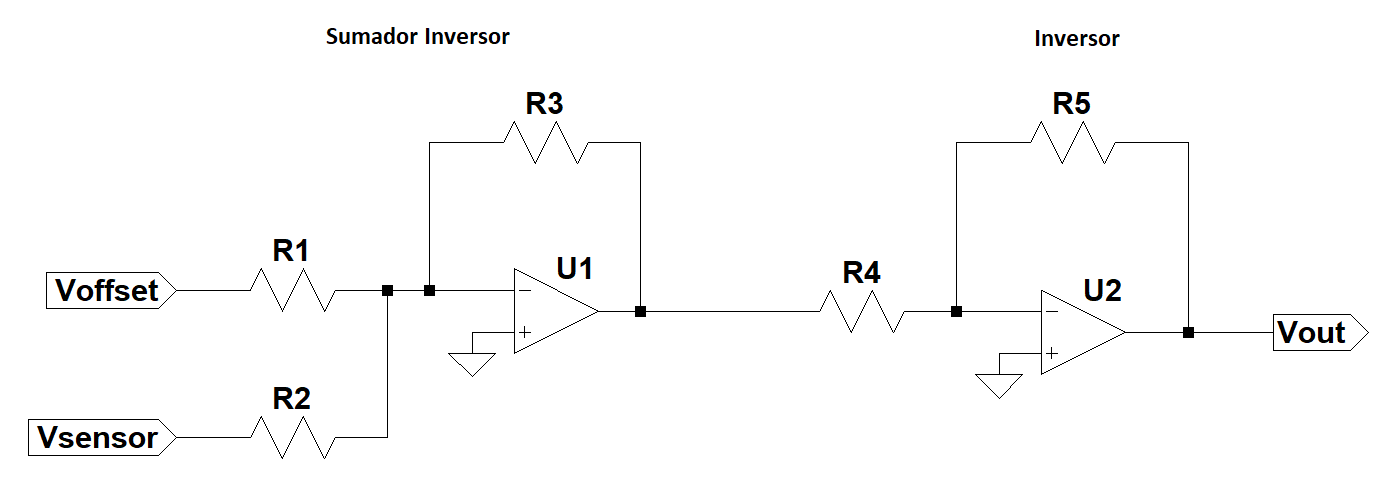
\includegraphics[width=0.9\textwidth]{../EJ_6/Captures/EJ6_circuito_teorico.png}
    \caption{Circuito adaptador}
    \label{fig:EJ6_circuito} 
\end{figure}

Dado que se utilizan dos amplificadores operacionales se creyó conveniente emplear el integrado TL082. La ecuación que caracteriza a dicho circuito se reproduce a continuación.

\begin{equation}
    v_{out}= \left( - \frac{R_3}{R_2} \cdot v_{sensor}  - \frac{R_3}{R_1} \cdot v_{offset} \right) \cdot \left( -\frac{R_5}{R_4}   \right)
    \label{fig:EJ6_ecuacion_sistema} 
\end{equation}

Si suponemos que el amplificador inversor tiene ganancia unitaria (esto es, $R_5=R_4$), y que la tensión que se usará como offset es $-V_{cc}$ obtenemos

\begin{equation}
    v_{out}= \frac{R_3}{R_2} \cdot v_{sensor}  - \frac{R_3}{R_1} \cdot v_{cc} 
    \label{fig:EJ6_ecuacion_sistema2} 
\end{equation}

En la ecuación anterior se pueden apreciar las dos etapas de adaptación mencionadas anteriormente (escalamiento y corrimiento). Ahora si operamos sobre esta simplificación obtenemos

\begin{equation}
    v_{out}= \frac{R_3}{R_2} \cdot \left( v_{sensor} - \frac{R_2}{R_1} \cdot v_{cc} \right)
    \label{fig:EJ6_ecuacion_sistema_simplificada_final} 
\end{equation}

Si decidimos fijar $R_2$ entonces agregando presets en serie a $R_1$ y $R_3$ podremos ajustar de forma independiente el corrimiento y escalamiento, respectivamente.
Realizando los c\'alculos apropiados para conocer los valores de los resistores se llega a la siguiente expresi\'on:

\begin{equation}
    R_1 = \frac{v_{cc} \cdot 50 \cdot R_2}{17.5}
    \label{fig:EJ6_ecuacion_resistores}
\end{equation}

\begin{equation}
  R_3 = 50 \cdot R_2
  \label{fig:EJ6_ecuacion_resistores2}
\end{equation}

Con las equivalencias anteriores y fijando un valor comercial para el resistor $R_2$ se pueden calcular los valores teóricos de resistencia para $R_1$ y $R_3$.
  Luego se normalizan estos valores, al valor comercial inmediato inferior que tambi\'en se encuentre disponible en el pa\~nol de la facultad.
  Por \'ultimo se agregan dos presets de $100k\Omega$ en serie a $R_1$ y $R_3$ para poder efectuar la calibraci\'on del circuito. Se obtiene la configuraci\'on que se detalla en la tabla de abajo.

  \begin{table}[H]
	\begin{center}
		\begin{tabular}{c c c c c}
		$R_2$ & $R_1$ & $R_{1n}$ & $R_3$ & $R_{3n}$ \\
		\hline
		$6.8 k\Omega$ & $291.49 k\Omega$ & $220 k\Omega + 100 k\Omega$ & $340 k\Omega$ & $270 k\Omega + 100 k\Omega$
		\end{tabular}
		
		\caption{Valores de resistores empleados}
	\end{center}
\end{table}

Los presets fueron sobredimensionados con el prop\'osito de ampliar el rango de calibraci\'on, de tal forma de compensar las tolerancias de los resistores (que en todos los casos es del 5\percent).
 De esta forma, se concluye la primera etapa del diseño del circuito.

 \subsection{Limitaci\'on del rango de salida}

 Se pide que la salida del circuito siempre pertenezca al rango $[-1V , 6V]$. Para lograr esto se puede colocar un diodo zener de $v_z = 5.6 V$ en paralelo a esta, limitando el rango de tensiones a $[-0.7V , 5.6V]$.
  El problema que se presenta en este caso es la limitación en corriente a la salida del integrado TL082. Si la intensidad es considerablemente alta se quemar\'a el IC. 
  Esta situaci\'on se puede evitar conectando una impedancia en serie a la salida, antes del diodo zener.


Seg\'un la datasheet del TL082 extra\'ida de la web de Texas Instruments, cuando el operacional tiene conectada a su salida una carga tal que $R_L \geq 2k\Omega$ puede hacer un swing m\'aximo de tensi\'on a la salida de $\v_{out} = pm10V$.
 Esta limitaci\'on est\'a dada por la corriente m\'axima que puede entregar en circuito integrado en estas condiciones. Aplicando ley de ohm se obtiene que en el peor caso

 \begin{equation}
    I_{max} = \frac{v_{max}}{R_L} = \frac{10V}{2k\Omega} = 5mA
    \label{fig:EJ6_ecuacion_corriente}
\end{equation}

Con esta corriente, y suponiendo ademas que el m\'odulo de la tensi\'on m\'axima de salida es menor a  $\v_{max} = 10V$ y que caen $5.6V$ sobre el zener, se calcula el resistor m\'inimo a ser colocado

\begin{equation}
    R_{min} = \frac{v_{max}-v_{z}}{I_{max}} = \frac{10V - 5.6V}{5mA} = 880\Omega
    \label{fig:EJ6_ecuacion_resistor_serie}
\end{equation}

Luego, se decidi\'o emplear un resistor cuyo valor nominal sea $1k\Omega$, de forma tal de agregar un factor de seguridad al circuito.
 Esta resistencia serie sumada a la impedancia de salida del circuito adaptador forman un divisor de tensi\'on que atenuar\'a la salida en un determivtinado valor. Esto se compensar\'a con el sobredimensionamiento de los presets de calibraci\'on.

 \subsection{Aspectos constructivos}

 Luego de la etapa de c\'alculo se procedi\'o al dise\~no propiamente dicho. En cuanto a conectividad, el PCB cuenta con una bornera de entrada con entrada triple y dos pares de pines de salida: uno que responde a la señal de salida del circuito, y otro que actúa como entrada de una señal de prueba que emula al sensor LM35.
  Esta \'ultima conexi\'on es especialmente \'util a la hora de realizar el proceso de calibraci\'on. Para poder conmutar entre la se\~nal simulada y la propia del sensor existe un jumper. A continuaci\'on se muestra un layout del PCB diseñado en Altium y una captura del esquem\'atico.
 
  \begin{figure}[H]
    \centering
    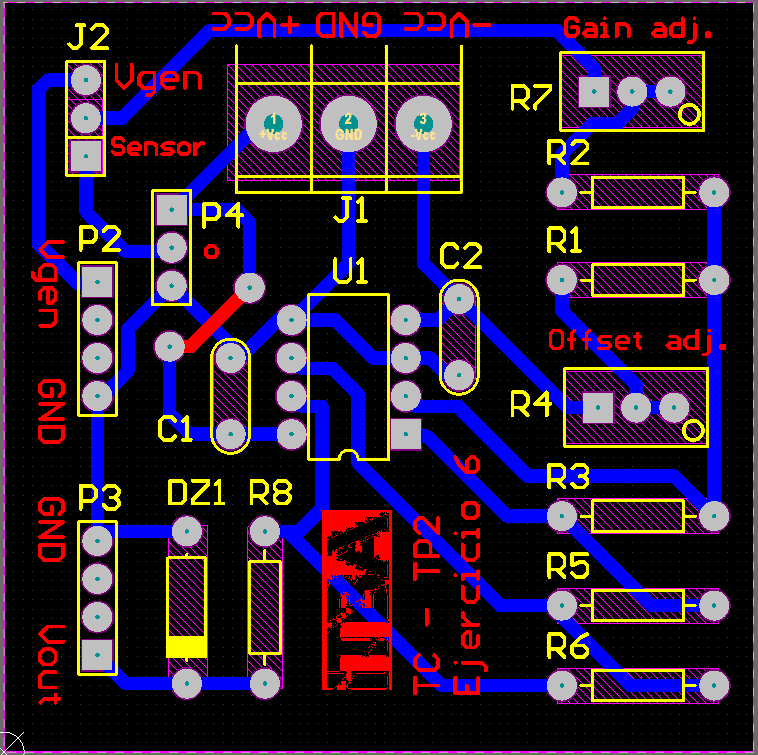
\includegraphics[width=0.9\textwidth]{../EJ_6/Captures/EJ6_PCB.png}
    \caption{PCB del circuito}
    \label{fig:EJ6_PCB} 
\end{figure}
 \subsection{M\'etodo de calibraci\'on}

 \begin{figure}[H]
    \centering
    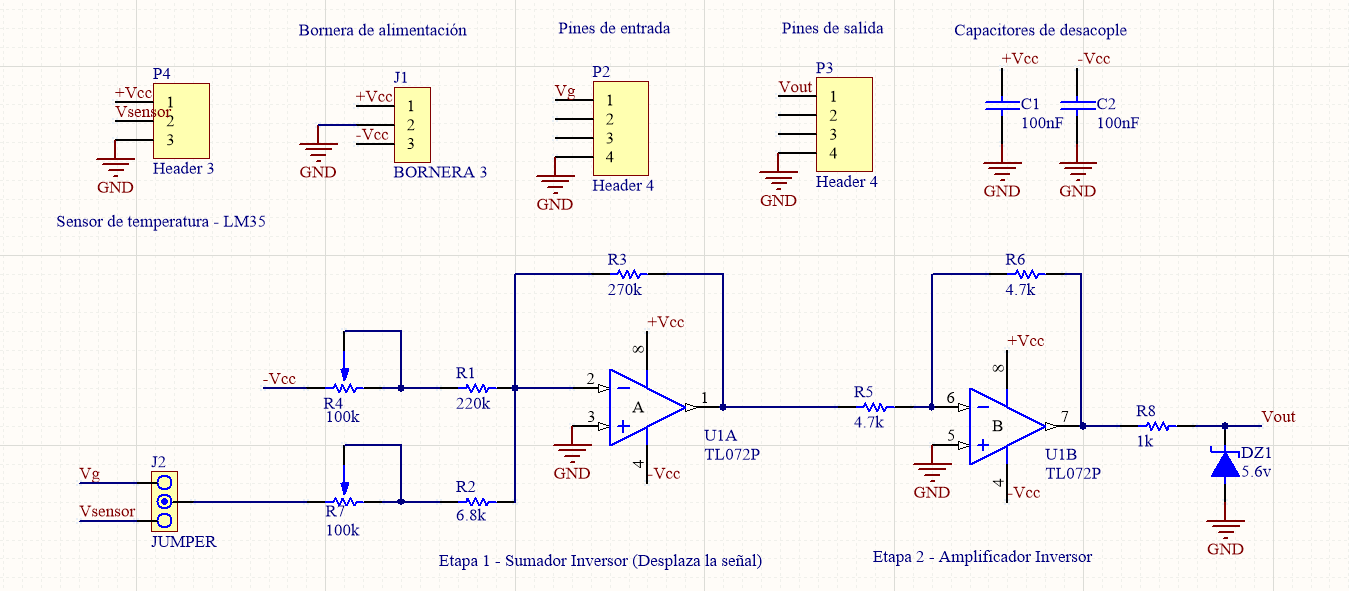
\includegraphics[width=0.9\textwidth]{../EJ_6/Captures/EJ6_schematic.png}
    \caption{Esquem\'atico del circuito}
    \label{fig:EJ6_schematic} 
\end{figure}

 \subsection{M\'etodo de calibraci\'on}

 Como se mencion\'o previamente, todos los componentes tienen una determinada tolerancia en sus valores nominales, adem\'as de ser \'estos normalizados y dependientes de factores externos como temperatura de operaci\'on, aging, etc.
  De esto se deriva la necesidad de implementar un m\'etodo de calibraci\'on que permita al circuito operar como lo esperado. El PCB cuenta con dos preset a tal fin, cuya funci\'on est\'a debidamente indicada en el mismo.
  Para realizar la calibraci\'on del circuito primero se recomienda conectar un generador de señales a la entrada para poder simular la respuesta del sensor en forma de rampa.
 Luego se debe conectar la salida a un osciloscopio y girar el preset de Offset hasta que el pico inferior de la rampa se sit\'ue en el cero. Una vez realizado esto se procede a girar el preset de ganancia hasta que el pico superior de la rampa alcance una tensi\'on de 5V.
  Cabe destacar que un proceso similar puede ser realizado con el sensor LM35 conectado e inyectando se\~al, utilizando la temperatuta de $35°C$ como referencia y otro punto dentro del rango.

  \subsection{Datasheet de la implementaci\'on}
    A continuaci\'on se reproducen algunos datos \'utiles del circuito.
    
  \begin{table}[]
    \begin{tabular}{c|ccc}
    \textbf{Item}                                    & \textbf{Min} & \textbf{Typ} & \textbf{Max} \\ \hline
    +Vcc {[}V{]}                                     & 5            & 15           & 36           \\
    -Vcc {[}V{]}                                     & -12          & -15          & -17          \\
    Vout {[}V{]}                                     & -0.8         & -            & 5.45         \\
    Amplitud de salida {[}V{]}                       & 3.92         & -            & 5.3          \\
    Impedancia de salida {[}\textbackslash{}Omega{]} & -            & 1000         & -            \\
    Amplificador Operacional                         & \multicolumn{3}{c|}{TL072CN}               \\
    Sensor de Temperatura                            & \multicolumn{3}{c|}{LM35DZ}               
    \end{tabular}
    \label{"Datasheet de la implementaci\'on"}
    \end{table}